




The decoupling approach~\cite{hayden2008decoupling, dupuis2010decoupling, Szehr2013decouple2design, dupuis2014one, preskill2016quantumshannon} and the Uhlmann transformation are combined and applied to various important tasks in quantum information processing.
We here consider two examples: entanglement transmission~\cite{Schumacher1996sendingentanglement, schumacher2001approximateerrorcorrection, hayden2007black, datta2013oneshotentassistQCcom, beigi2016decoding, khatri2024principlemodern} and quantum state merging~\cite{Horodecki2005Partialquantinfo, berta2008singleshot, dupuis2014one, yamasaki2019statemergesmalldimension}.

We employ our algorithms to perform the Uhlmann transformation in these tasks and evaluate the computational cost.
Since these tasks typically involve tripartite or multipartite states, some adjustments are often required beyond the direct application of our Uhlmann transformation algorithms.
For discussions on the optimality of the Uhlmann transformation in the cases involving tripartite or multipartite states, see \Cref{sec:opt local and Uhlmann}.

In \Cref{sec:general decoup and Uhl}, we overview the decoupling and the Uhlmann transformation. In \Cref{sec:qi transmission}, we discuss one-shot entanglement transmission and analyze the computational costs when we use our Uhlmann transformation algorithms. 
In \Cref{sec:entdis and uhl}, we address one-shot quantum state merging and also evaluate the computational costs of our algorithms.


In this section and subsequent sections, we use the following notation.
We denote the completely mixed state by $\pi$, such as $\pi^\sA = \mathbb{I}^\sA/d_\sA$ for system $\sA$, and denote by $U_\Phi$ a unitary that prepares a maximally entangled state: $U_\Phi^{\sA\sA'}\ket{0}^{\sA\sA'} = \ket{\Phi}^{\sA\sA'}$.
While we usually denote a pure state as $\ket{\omega}$, the corresponding density matrix is sometimes written as $\omega = \ketbra{\omega}{\omega}$. For instance, the density matrix of a pure state $\ket{\omega}^{\sA\sB}$ is denoted by $\omega^{\sA\sB}$.

%======================================================================================================================================================




\subsection{Decoupling and Uhlmann's theorem}
\label{sec:general decoup and Uhl}


The decoupling is a standard approach, often combined with the Uhlmann transformation, that characterizes information-theoretic limits of information tasks.
The key idea of the decoupling is to estimate how much quantum information is leaked to an ``environment'' of a quantum channel. This is specifically quantified by the degree of decoupling.


For a quantum channel $\cF^{\sA\rarr\sC}$, let $V_\cF^{\sA \rarr \sC\sE}$ be a Stinespring isometry~\cite{stinespring1955} of $\cF^{\sA \rarr \sC}$ by an environment $\sE$.
That is, $V_\cF^{\sA \rarr \sC\sE}$ is such that $\cF^{\sA\rarr \sC}$ is represented as $\cF^{\sA \rarr \sC}(\cdot) = \tr_{\sE}\big[V_\cF^{\sA\rarr \sC\sE}(\cdot)(V_\cF^{\sA \rarr \sC\sE})^\dag\big]$.
A complementary channel $\bar{\cF}^{\sA\rarr\sE}$ is defined by $\bar{\cF}^{\sA\rarr\sE}(\cdot) = \tr_\sC\big[V_\cF^{\sA\rarr\sC\sE}(\cdot)(V_\cF^{\sA\rarr\sC\sE})^\dag\big]$.
Note that the Stinespring isometry $V_\cF^{\sA \rarr \sC\sE}$ and the complementary channel $\bar{\cF}^{\sA\rarr\sE}$ are not uniquely determined by $\cF^{\sA\rarr \sC}$; there is freedom to apply an additional isometry on the environment $\sE$.

The decoupling approach is described as follows: suppose that for a pure state $\ket{\omega}^{\sR\sA\sB}$ with a reference system $\sR$ and $\epsilon \in [0, 1]$, there exists a state $\tau^\sE$ such that 
\begin{align}
\label{eq:decoup cond}
    \rF\big(\bar{\cF}^{\sA\rarr\sE}(\omega^{\sR\sA}), \omega^\sR \otimes \tau^\sE\big) \geq 1 - \epsilon.
\end{align}
Then, there is the Uhlmann unitary $V^\sM$ on $\sM = \sB\sC\sD = \hat{\sA}\hat{\sB}\hat{\sE}$
that satisfies
\begin{align}
    \rF\big(V^\sM V_\cF^{\sA\rarr\sC\sE}\ket{\omega}^{\sR\sA\sB}\ket{0}^\sD, \ket{\omega}^{\sR\hat{\sA}\hat{\sB}}\ket{\tau}^{\sE\hat{\sE}}\big)
    &= \rF\big(\bar{\cF}^{\sA\rarr\sE}(\omega^{\sR\sA}), \omega^\sR \otimes \tau^\sE\big) \\
    \label{inteq:80}
    &\geq 1 - \epsilon,
\end{align}
where $\ket{\tau}^{\sE\hat{\sE}}$ is a purified state of $\tau^\sE$.
This implies that, if $\epsilon$ is sufficiently small, one can approximately obtain the state  $\ket{\omega}^{\sR\hat{\sA}\hat{\sB}}\ket{\tau}^{\sE\hat{\sE}}$, by acting only on $\sB\sC\sD$ of the state 
$V_\cF^{\sA\rarr\sC\sE}\ket{\omega}^{\sR\sA\sB}\ket{0}^\sD$,
without manipulating $\sR\sE$.
The inequality in Eq.~\eqref{eq:decoup cond} is known as the \emph{decoupling condition}, which evaluates how well the reference system $\sR$ and the environment $\sE$ are decoupled, with the parameter $\epsilon$ quantifying the degree of decoupling.





The decoupling approach is applicable to a wide range of information-processing tasks.
In particular, the case where $\cF^{\sA\rarr\sC}$ is given by $\cF^{\sA\rarr\sC} = \cG^{\sA\rarr\sC} \circ \cU^\sA$ with a \emph{Haar random unitary} $U^\sA$ and some quantum channel $\cG^{\sA\rarr\sC}$ is often considered.
In this case, \emph{decoupling theorem}~\cite{dupuis2014one} states that $\epsilon$ in the decoupling condition can be taken sufficiently small with high probability for $\tau^\sE = \bar{\cG}^{\sA\rarr\sE}(\pi^\sA)$, depending on a certain entropy condition specified by the initial state $\ket{\omega}^{\sR\sA\sB}$ and the channel $\cG^{\sA\rarr\sC}$.
Here, $\bar{\cG}^{\sA\rarr\sE}(\pi^\sA)$ is a reduced state on $\sE$ of the \emph{Choi–Jamio\l kowski state} $\bar{\cG}^{\sA\rarr\sE}(\Phi^{\sR\sA})$ of $\bar{\cG}^{\sA\rarr\sE}$.
The dependence of $\epsilon$ on $\ket{\omega}^{\sR\sA\sB}$ and $\cG^{\sA\rarr\sC}$ via the entropy condition plays a key role in deriving the theoretical limits of some tasks, such as the quantum capacity~\cite{hayden2008decoupling}.
Yet we do not address this dependence explicitly here, as it is not crucial in our discussion (for details, see, e.g., Refs.~\cite{dupuis2010decoupling, dupuis2014one, khatri2024principlemodern}).




Henceforth, following this convention, we use a Haar random unitary $U^\sA$ and fix $\tau^\sE$ as $\tau^\sE = \bar{\cG}^{\sA\rarr\sE}(\pi^\sA)$.
We remark that even if the Haar random unitary in these tasks is replaced by a unitary 2-design for practical purposes, a similar discussion holds~\cite{Szehr2013decouple2design}.
Unlike the Haar random unitary, the unitary 2-design can be realized efficiently as quantum circuits, e.g., using the Clifford group~\cite{DiVincenzoQdatahiding}, near-linear construction~\cite{cleve2016nearlinearexact2design}, or random unitaries diagonal in the Pauli-$Z$ and -$X$ bases~\cite{Nakata2017randomdiagonal2design}.






%==========================================================================================================================================





\subsection{One-shot entanglement transmission}
\label{sec:qi transmission}





An important application of the decoupling and the Uhlmann's theorem is entanglement transmission.
We describe the setting in \Cref{seq:setting of ent transmission}, and then, in \Cref{sec:analyze of uhl alg in ent trans}, we investigate the implementation of the Uhlmann transformation for entanglement transmission, based on our algorithm.




\subsubsection{Setting}
\label{seq:setting of ent transmission}

Alice aims to send a system $\sA$ of a maximally entangled state $\ket{\Phi}^{\sR\sA}$ to Bob through a noisy quantum channel, where $d_\sR = d_\sA$.
They may share $(\log{d_\sG})$-ebit entanglement $\ket{\Phi}^{\sG\hat{\sG}}$ in advance, which can be used in the encoding and decoding processes, where $\sG$ is held by Alice and $\hat{\sG}$ by Bob.
When $d_\sG=1$, it is the entanglement-non-assisted setting; otherwise, the entanglement-assisted setting.
Alice encodes the system $\sA$ together with $\sG$ using a Haar random unitary $U^{\sA\sG}$, then sends $\sA\sG$ through a noisy quantum channel $\cN^{\sA\sG\rarr\sB}$ to Bob.
After receiving the system $\sB$, Bob applies a decoding map $\cD^{\sB\hat{\sG}\rarr\hat{\sA}}$.
See also \Cref{fig:diagram of QI transmitt}.


We denote by $\bar{\cN}^{\sA\sG\rarr\sE}$ a complementary channel of $\cN^{\sA\sG\rarr\sB}$, where $\sE$ is an environment.
The decoupling theorem~\cite{dupuis2014one} guarantees that an encoding Haar random unitary $U^{\sA\sG}$ satisfies with high probability that 
\begin{align}
\label{inteq:102}
    \rF\big(\bar{\cN}^{\sA\sG\rarr\sE}\circ\cU^{\sA\sG}(\Phi^{\sR\sA} \otimes \pi^\sG), \pi^\sR \otimes \tau^\sE\big) \geq 1 - \epsilon,
\end{align}
where $\tau^\sE = \bar{\cN}^{\sA\sG\rarr\sE}(\pi^{\sA\sG})$.
The parameter $\epsilon$ depends on the channel $\cN^{\sA\sG\rarr\sB}$ and the number of pre-shared ebits.
Note that Eq.~\eqref{inteq:102} holds independently of the choice of the complementary channel of $\cN^{\sA\sG\rarr\sB}$, as the complementary channel has the freedom to apply an additional isometry on $\sE$ and the fidelity is invariant under such an isometry.



Due to Eq.~\eqref{inteq:80}, there is a quantum channel $\cD^{\sB\hat{\sG} \rarr \hat{\sA}} = \tr_{\hat{\sE}} \circ \cV^\sM \circ \cP_{\ket{0}}^{\bC \rarr \sD}$, where $\sM = \sB\hat{\sG}\sD = \hat{\sA}\hat{\sE}$ and $V^\sM$ is the Uhlmann unitary, which satisfies
\begin{align}
\label{inteq:101}
    \rF\big(\cD^{\sB\hat{\sG} \rarr \hat{\sA}}\circ \cN^{\sA\sG \rarr \sB} \circ \cU^{\sA\sG} (\Phi^{\sR\sA} \otimes \Phi^{\sG\hat{\sG}}), \ket{\Phi}^{\sR\hat{\sA}}\big) \geq 1 - \epsilon,
\end{align}
where we used Eq.~\eqref{inteq:102}.
This implies that, under the condition that $\sR$ and $\sE$ are sufficiently decoupled in the sense of Eq.~\eqref{inteq:102} with small $\epsilon$, Bob can recover the original maximally entangled state $\ket{\Phi}^{\sR\sA}$ from the output of the noisy channel $\cN^{\sA\sG\rarr\sB}$ by applying $\cD^{\sB\hat{\sG}\rarr\hat{\sA}}$, succeeding in transmitting entanglement from Alice to Bob.
We call this quantum channel $\cD^{\sB\hat{\sG}\rarr\hat{\sA}}$ the \emph{Uhlmann decoder}.



\begin{figure}
    \centering
    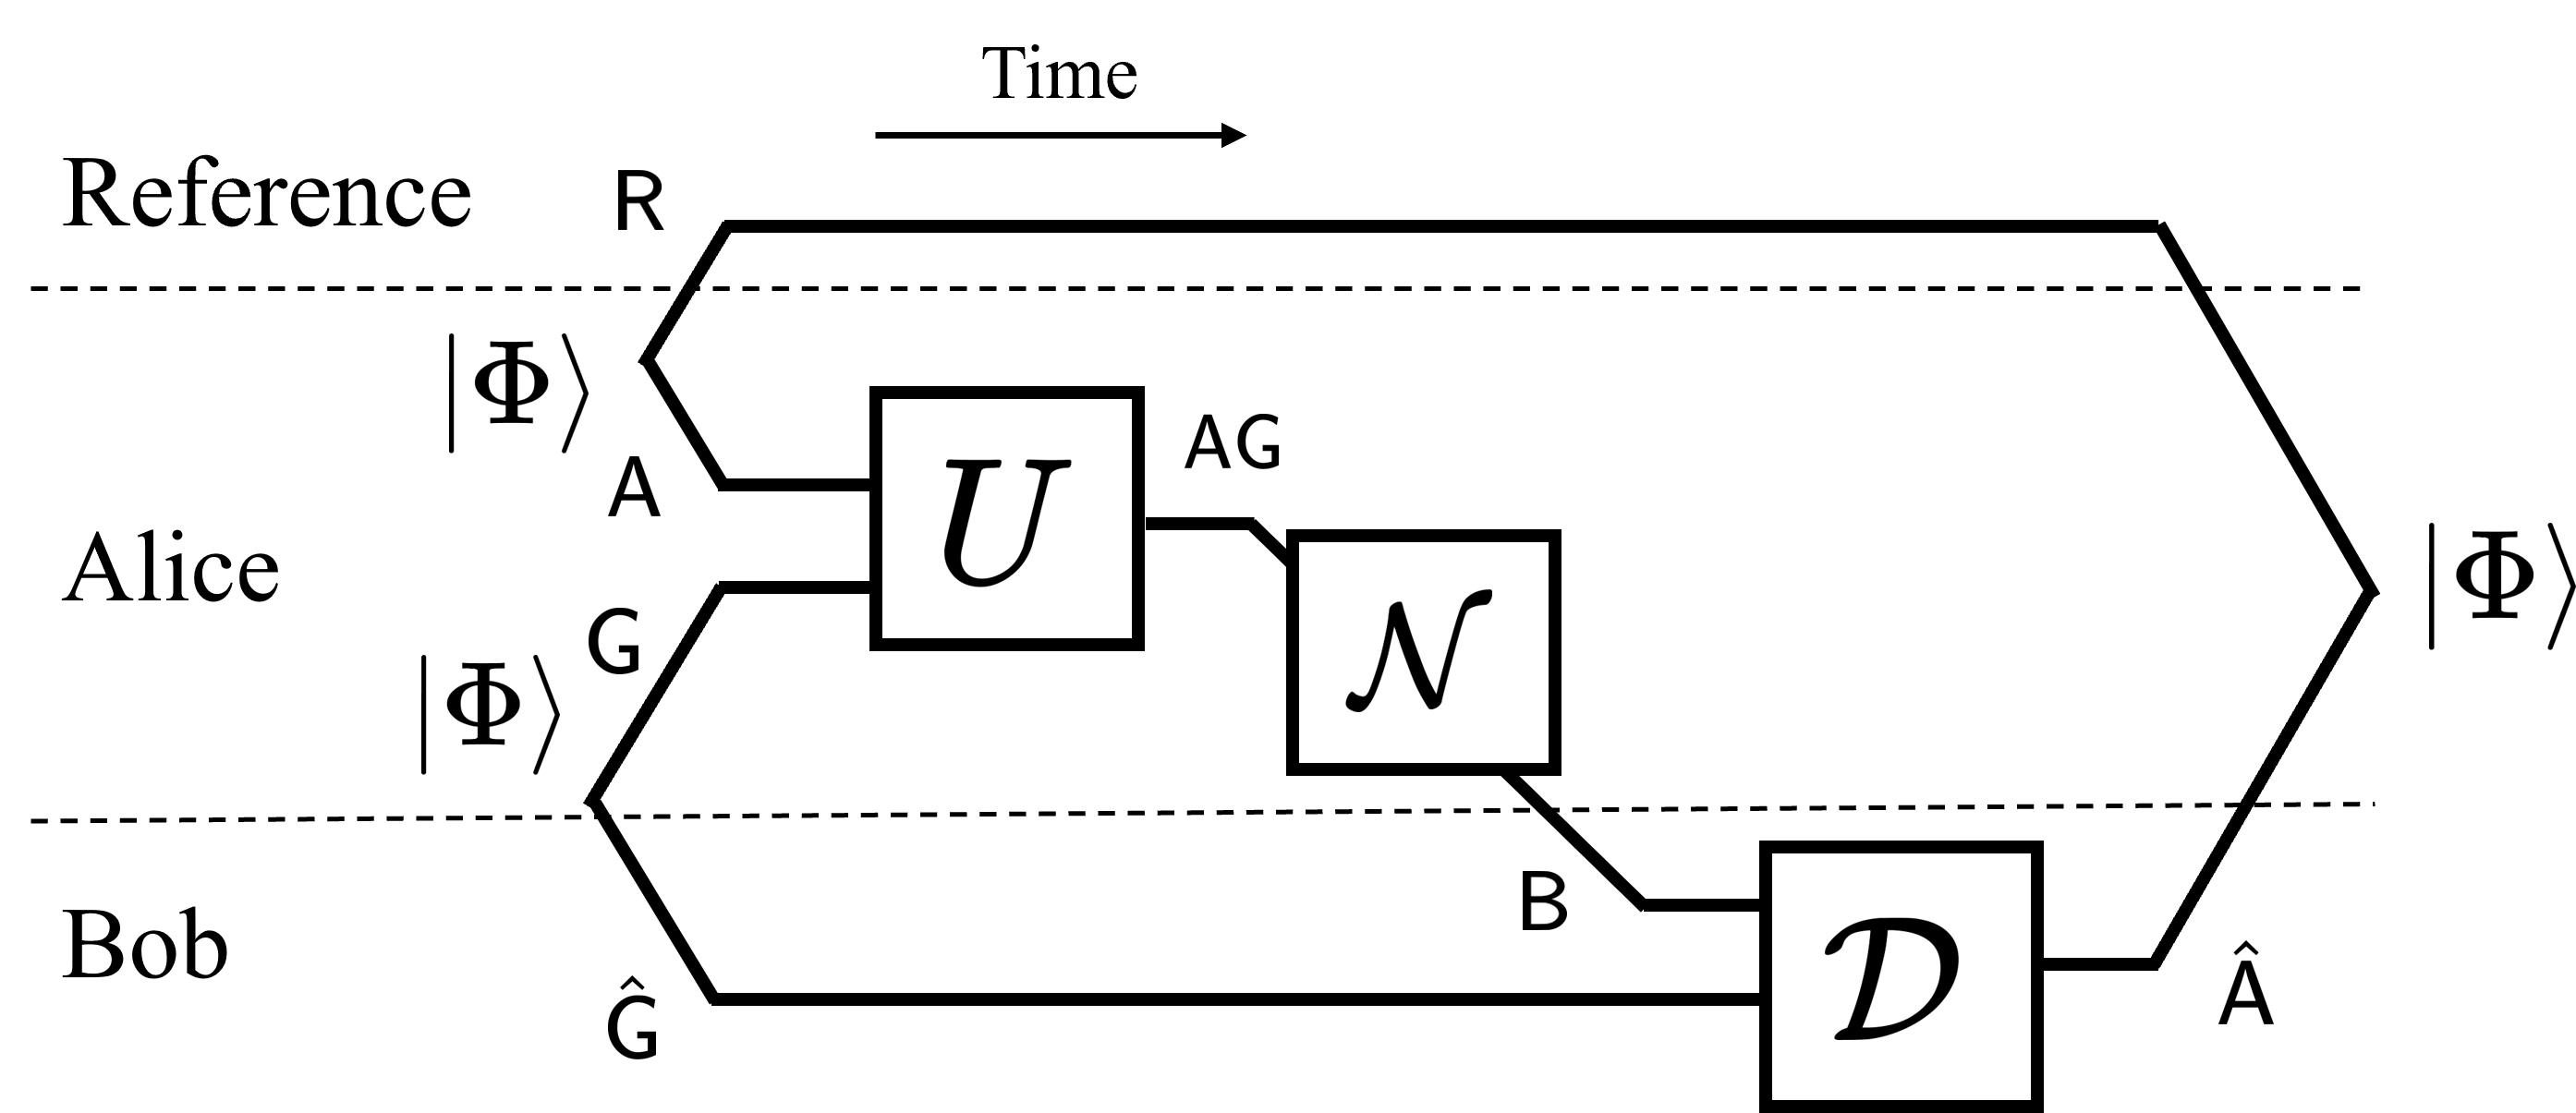
\includegraphics[width=100mm]{fig3.png}
    \caption{A diagram of entanglement transmission. 
    Alice applies a Haar random unitary $U^{\sA\sG}$ to encode $\sA$ with $\sG$, which is part of a possibly pre-shared entangled state $\ket{\Phi}^{\sG\hat{\sG}}$. Alice then transmits $\sA\sG$ to Bob through a noisy quantum channel $\cN^{\sA\sG\rarr\sB}$.
    After receiving $\sB$, Bob applies a decoding map $\cD^{\sB\hat{\sG}\rarr\hat{\sA}}$ on $\sB\hat{\sG}$ to obtain a final state that approximates the maximally entangled state $\ket{\Phi}^{\sR\hat{\sA}}$.}
    \label{fig:diagram of QI transmitt}
\end{figure}





%=====================================================================================================================================================================================================================================


\subsubsection{Algorithmic implementation of the Uhlmann decoder}
\label{sec:analyze of uhl alg in ent trans}


We consider that Bob implements the Uhlmann decoder using our algorithm.
We assume that Bob knows Alice's operation $U^{\sA\sG}$ and is capable of applying it.
It is standard in decoding to assume that Bob knows how Alice encoded the system.
Even if $U^{\sA\sG}$ is chosen uniformly at random, Bob can determine which unitary was applied, for example, using shared randomness with Alice.
Let $U_\cN^{\sS}$ be a Stinespring unitary on $\sS = \sA\sG\sC = \sB\sE$, i.e., $U_\cN^{\sS}\ket{0}^{\sC} = V_\cN^{\sA\sG\rarr\sB\sE}$, where $V_\cN^{\sA \to \sB\sE}$ is a Stinespring isometry of $\cN^{\sA \to \sB}$.
For algorithmic construction, we consider two different models: 
\begin{enumerate}
    \item A model in which multiple uses of a Stinespring unitary $U_\cN^{\sS'}$ are available.
    \item A model in which multiple uses of the quantum channel $\cN^{\sA'\sG' \to \sB'}$ are available.
\end{enumerate}
We evaluate the number of uses of $U_\cN^{\sS'}$ or $\cN^{\sA'\sG'\rarr\sB'}$ by Bob to implement the Uhlmann decoder in each model.
Note that we should distinguish between the existing systems, such as $\sR$ and $\sS$, and the systems subsequently prepared and simulated by Bob, e.g., $\sS'$.





We define two pure states $\ket{\Psi}^{\sR\sB\hat{\sG}\sE}$ and $\ket{\tau}^{\sR\sB\hat{\sG}\sE}$ as 
\begin{align}
    \ket{\Psi}^{\sR\sB\hat{\sG}\sE} = V_\cN^{\sA\sG\rarr\sB\sE} U^{\sA\sG} \ket{\Phi}^{\sR\sA}\ket{\Phi}^{\sG\hat{\sG}}, \ \ \ \text{and} \ \ \
    \ket{\tau}^{\sR\sB\hat{\sG}\sE} = V_\cN^{\sA\sG\rarr\sB\sE}\ket{\Phi}^{\sR\sA}\ket{\Phi}^{\sG\hat{\sG}}.
\end{align}
For a matrix $A$, we use $\lambda_{\rm min}(A)$ and $r(A)$ to denote the minimum non-zero eigenvalue and the rank of $A$, respectively.
Our statement is as follows, where $\mu_{\rm min}$ is given by $\mu_{\rm min} = \sqrt{\lambda_{\rm min}(\Psi^{\sB\hat{\sG}})\lambda_{\rm min}(\tau^{\sB\hat{\sG}})/d_\sA}$.

\begin{theorem}[Algorithmic implementation of the Uhlmann decoder]
\label{thm:Uhlmann decoder ent trans}
    In the setting of entanglement transmission, suppose that an encoding unitary $U^{\sA\sG}$ satisfies
    \begin{align}
    \label{inteq:136}
        \rF\big(\bar{\cN}^{\sA\sG\rarr\sE}\circ\cU^{\sA\sG}(\Phi^{\sR\sA} \otimes \pi^\sG), \pi^\sR \otimes \tau^\sE\big) \geq 1 - \epsilon,
    \end{align}
    for some $\epsilon \in [0, 1]$ and $\tau^\sE = \bar{\cN}^{\sA\sG\rarr\sE}(\pi^{\sA\sG})$.
    Then, for $\delta \in (0, 1)$, there exists a quantum algorithm that implements a quantum channel $\til{\cD}^{\sB\hat{\sG}\rarr\hat{\sA}}$, which satisfies
    \begin{align}
    \label{inteq:157}
        \rF\big(\til{\cD}^{\sB\hat{\sG} \rarr \hat{\sA}}(\Psi^{\sR\sB\hat{\sG}}), \ket{\Phi}^{\sR\hat{\sA}}\big) \geq 1 - \epsilon -\delta,
    \end{align}
    using, in Model~1: 
    \begin{align}
    \label{inteq:121}
        \cO\Big(\min\Big\{\f{1}{\mu_{\rm min}}, \f{r(\Psi^{\sB\hat{\sG}})}{\delta}\Big\}\log{\Big(\f{1}{\delta}\Big)}\Big)
    \end{align}
    of a Stinespring unitary $U_\cN^{\sS'}$ or, 
    in Model~2: 
    \begin{align}
    \label{inteq:137}
        \til{\cO}\Big(\f{d_\sA d_\sB d_\sG}{\delta^2 \mu_{\rm min}^3} \min\Big\{\f{1}{\lambda_{\rm min}^2(\Psi^{\sR\sB\hat{\sG}})} + \f{1}{\lambda_{\rm min}^2(\tau^{\sR\sB\hat{\sG}})}, \f{d_\sA^2 d_\sB^2 d_\sG^2}{\delta^4 \mu_{\rm min}^4}\Big\}\Big)
    \end{align}
    of the quantum channel $\cN^{\sA'\sG'\rarr\sB'}$.
    In both models, $\cO\big(\log{(d_\sA d_\sB d_\sG)}\big)$ qubits suffice at any one time.
\end{theorem}



In each model, if one is interested in the circuit complexity, it can be estimated to the leading order by multiplying the number of one- and two-qubit gates for implementing $U_\cN^{\sS'}$ or $\cN^{\sA'\sG'\rarr\sB'}$ by the respective number of times they are used, given in Eq.~\eqref{inteq:121} and Eq.~\eqref{inteq:137}.



Before proceeding to the proof of Theorem~\ref{thm:Uhlmann decoder ent trans}, we briefly compare the number of uses of $U_\cN^{\sS'}$ in Eq.~\eqref{inteq:121} with those of existing decoders, the generalized Yoshida-Kitaev decoder, and the Petz-like decoder~\cite{utsumi2024explicitdecoderQSVTt}.
The number of uses of $U_\cN^{\sS'}$ in these decoders is given by
\begin{align}
\label{inteq:82}
    \cO\Big(\sqrt{d_\sB/\big(d_\sG\lambda_{\rm min}(\Psi^{\sB\hat{\sG}})\big)}\log{(1/\delta)}\Big),
\end{align}
for the generalized Yoshida-Kitaev decoder, and
\begin{align}
\label{inteq:83}
    \cO\Big(\sqrt{d_\sE/\big(d_\sA\lambda_{\rm min}(\Psi^{\sB\hat{\sG}})\big)} \log{(1/\delta)}\Big),
\end{align}
for the Petz-like decoder.
From the comparison of Eqs.~\eqref{inteq:121} and~\eqref{inteq:82}, we see that if an inequality 
\begin{align}
    \f{d_\sG}{d_\sB}\min\Big\{\f{d_\sA}{\lambda_{\rm min}(\tau^{\sB\hat{\sG}})}, \f{1}{\delta^2}\Big\} \leq 1,
\end{align}
is satisfied, the Uhlmann decoder can be implemented more efficiently than the generalized Yoshida-Kitaev one, where we used the relation $r(\Psi^{\sB\hat{\sG}}) \leq 1/\lambda_{\rm min}(\Psi^{\sB\hat{\sG}})$.
Similarly, comparing Eqs.~\eqref{inteq:121} and~\eqref{inteq:83}, we observe that when $\f{d_\sE}{d_\sA}\min\Big\{\f{d_\sA}{\lambda_{\rm min}(\tau^{\sB\hat{\sG}})}, \f{1}{\delta^2}\Big\} \leq 1$, the Uhlmann decoder can be implemented more efficiently than the Petz-like decoder.









\begin{proof}[Proof of Theorem~\ref{thm:Uhlmann decoder ent trans}]
    

We first consider Model~1.


We note that the states $\ket{\Psi}^{\sR\sB\hat{\sG}\sE}\ket{0}^{\hat{\sR}\hat{\sA}}$ and $\ket{\Phi}^{\sR\hat{\sA}}\ket{\tau}^{\hat{\sR}\sB\hat{\sG}\sE}$ are rephrased as 
$\ket{\Psi}^{\sR\sB\hat{\sG}\sE}\ket{0}^{\hat{\sR}\hat{\sA}} = W_\cN^{\sR\sS\hat{\sG}\hat{\sR}\hat{\sA}}\ket{0}^{\sR\sS\hat{\sG}\hat{\sR}\hat{\sA}}$ and $\ket{\Phi}^{\sR\hat{\sA}}\ket{\tau}^{\hat{\sR}\sB\hat{\sG}\sE} = \til{W}_\cN^{\sR\sS\hat{\sG}\hat{\sR}\hat{\sA}}\ket{0}^{\sR\sS\hat{\sG}\hat{\sR}\hat{\sA}}$, where
\begin{align}
    W_\cN^{\sR\sS\hat{\sG}\hat{\sR}\hat{\sA}} = U_\cN^{\sS}U^{\sA\sG}(U_\Phi^{\sR\sA}\otimes U_\Phi^{\sG\hat{\sG}})\otimes \bI^{\hat{\sR}\hat{\sA}}, \ \ \text{and} \ \ \ 
    \til{W}_\cN^{\sR\sS\hat{\sG}\hat{\sR}\hat{\sA}} = U_\Phi^{\sR\hat{\sA}} \otimes U_\cN^{\sS}(U_\Phi^{\hat{\sR}\sA}\otimes U_\Phi^{\sG\hat{\sG}}),
\end{align}
$U_\Phi\ket{0} = \ket{\Phi}$, and $\sS = \sA\sG\sC = \sB\sE$.
Using
\begin{align}
    \mathtt{UhlmannPurifiedQuery}(W_\cN^{\sR'\sS'\hat{\sG}'\hat{\sR}'\hat{\sA}'}, \til{W}_\cN^{\sR'\sS'\hat{\sG}'\hat{\sR}'\hat{\sA}'}; \delta, \tF),
\end{align}
described in \Cref{alg:Uhl purif query}, we can implement a quantum channel $\cT^\sM$ on $\sM = \sB\hat{\sG}\hat{\sR}\hat{\sA}$, which approximates the Uhlmann transformation and satisfies
\begin{align}
    \rF\big(\cT^\sM(\ketbra{\Psi}{\Psi}^{\sR\sB\hat{\sG}\sE}\otimes\ketbra{0}{0}^{\hat{\sR}\hat{\sA}}), \ket{\Phi}^{\sR\hat{\sA}}\ket{\tau}^{\hat{\sR}\sB\hat{\sG}\sE}\big)
    &\geq \rF(\Psi^{\sR\sE}, \pi^\sR\otimes\tau^\sE) -\delta \\
    &\geq 1-\epsilon - \delta,
\end{align}
where we used Theorem~\ref{thm:Uhlmann alg purif query model} and the decoupling condition Eq.~\eqref{inteq:136}.
Note that $\Psi^{\sR\sE} = \bar{\cN}^{\sA\sG\rarr\sE}\circ\cU^{\sA\sG}(\Phi^{\sR\sA} \otimes \pi^\sG)$.
From the monotonicity of the fidelity, a quantum channel $\til{\cD}^{\sB\hat{\sG}\rarr\hat{\sA}} = \tr_{\sB\hat{\sG}\hat{\sR}}\circ\cT^\sM \circ \cP_{\ket{0}}^{\bC\rarr\hat{\sR}\hat{\sA}}$ serves as a decoder such that
\begin{align}
    &\rF(\til{\cD}^{\sB\hat{\sG}\rarr\hat{\sA}}(\Psi^{\sR\sB\sG}), \ket{\Phi}^{\sR\hat{\sA}}) 
    \geq 1 - \epsilon - \delta.
\end{align}


The number of uses of $U_\cN^{\sS'}$ for applying the channel $\til{\cD}^{\sB\hat{\sG}\rarr\hat{\sA}}$, especially $\cT^\sM$, can be evaluated by Theorem~\ref{thm:Uhlmann alg purif query model} as
\begin{align}
\label{inteq:81}
    \cO\big(\min\{{1/s_{\rm min}}, r/\delta\}\log{(1/\delta)}\big), 
\end{align}
where $s_{\rm min}$ and $r$ are the minimum non-zero singular value and the rank of $\sqrt{\Psi^{\sR\sE}}\big(\sqrt{\pi^\sR}\otimes\sqrt{\tau^\sE}\big)$, respectively.

By applying the following two inequalities:
\begin{align}
    \label{inteq:138}
    &1/s_{\rm min} \leq \sqrt{d_\sA/\big(\lambda_{\rm min}(\Psi^{\sB\hat{\sG}})\lambda_{\rm min}(\tau^{\sB\hat{\sG}})\big)} = 1/\mu_{\rm min},  \\
    \label{inteq:139}
    &r \leq r(\Psi^{\sB\hat{\sG}}),
\end{align}
to Eq.~\eqref{inteq:81}, we finally obtain Eq.~\eqref{inteq:121}.
The inequalities follow from the so-called support lemma~\cite{Renner05securityQKD, wilde2013QItheory}: for any positive-semidefinite matrix $S^{\sA\sB}$, $\supp[S^{\sA\sB}] \subset \supp[S^\sA\otimes S^\sB]$.
By combining this fact with \Cref{prop:min singular inequality} in \Cref{sec:appendix product of singvalue}, Eq.~\eqref{inteq:138} is obtained.
Here, we note that $\tr_\sE[\Psi^{\sR\sE}] = \pi^\sR$ and $\tr_\sR[\Psi^{\sR\sE}] = \tau^\sE$.
The inequality in Eq.~\eqref{inteq:139} results from the rank of a product of matrices being at most the rank of each matrix.
Since $\supp[\Psi^{\sR\sE}] \subset \supp[\pi^\sR \otimes \tau^\sE]$, we have $\min\{r(\Psi^{\sR\sE}), r(\pi^\sR\otimes \tau^\sE)\} = r(\Psi^{\sR\sE})$.
Note that $\ket{\Psi}^{\sR\sB\hat{\sG}\sE}$ is a pure state, which implies $r(\Psi^{\sR\sE}) = r(\Psi^{\sB\hat{\sG}})$.







Next, we consider Model~2.
In this model, we need to obtain purified states, using a purification algorithm such as the canonical purification algorithm in \Cref{alg:canonical purification}.
Since the input state to the decoder does not depend on the choice of the environment $\sE$, for canonical purification, we set $\sE$ as $\sE = \sR''\sB''\hat{\sG}''$.




In contrast to Model~1, the construction of a decoder in Model~2 requires careful analysis, because considering a specific purification fixes the freedom in the environment of the channel $\cN^{\sA\sG\rarr\sB}$.
We explain the issue and its resolution below. 




The canonical purified states of
\begin{align}
\label{inteq:11}
    \Psi^{\sR\sB\hat{\sG}} = \cN^{\sA\sG\rarr\sB}\circ\cU^{\sA\sG}(\Phi^{\sR\sA}\otimes\Phi^{\sG\hat{\sG}}), \ \ \ \text{and} \ \ \ \tau^{\sR\sB\hat{\sG}} = \cN^{\sA\sG\rarr\sB}(\Phi^{\sR\sA}\otimes\Phi^{\sG\hat{\sG}}),
\end{align}
are given by 
\begin{align}
    &\ket{\Psi_{\rm c}}^{\sR\sB\hat{\sG}\sR''\sB''\hat{\sG}''} = \sqrt{\Psi^{\sR\sB\hat{\sG}}}\ket{\Gamma}^{\sR\sB\hat{\sG}\sR''\sB''\hat{\sG}''}, \label{Eq:PsiCanonical} \\
    &\ket{\tau_{\rm c}}^{\sR\sB\hat{\sG}\sR''\sB''\hat{\sG}''} = \sqrt{\tau^{\sR\sB\hat{\sG}}}\ket{\Gamma}^{\sR\sB\hat{\sG}\sR''\sB''\hat{\sG}''},
\end{align}
respectively, where $\ket{\Gamma}^{\sR\sB\hat{\sG}\sR''\sB''\hat{\sG}''}$ is the unnormalized maximally entangled state between $\sR\sB\hat{\sG}$ and $\sR''\sB''\hat{\sG}''$.
The Stinespring isometry $V_{\cN, \tau_{\rm c}}^{\sA\sG\rarr\sB\sR''\sB''\hat{\sG}''}$ of $\cN^{\sA\sG\rarr\sB}$, determined from $\ket{\tau_{\rm c}}^{\sR\sB\hat{\sG}\sR''\sB''\hat{\sG}''}$, satisfies
\begin{align}
\label{inteq:66}
    \ket{\tau_{\rm c}}^{\sR\sB\hat{\sG}\sR''\sB''\hat{\sG}''} 
    = V_{\cN, \tau_{\rm c}}^{\sA\sG\rarr\sB\sR''\sB''\hat{\sG}''}\ket{\Phi}^{\sR\sA}\ket{\Phi}^{\sG\hat{\sG}}.
\end{align}



To see how $V_{\cN, \tau_{\rm c}}^{\sA\sG\rarr\sB\sR''\sB''\hat{\sG}''}$ is related to the Stinespring isometry determined from $\ket{\Psi_{\rm c}}^{\sR\sB\hat{\sG}\sR''\sB''\hat{\sG}''}$, we note that Eqs.~\eqref{inteq:11} imply $\Psi^{\sR\sB\hat{\sG}} = (U^{\sR\hat{\sG}})^\top\tau^{\sR\sB\hat{\sG}}(U^{\sR\hat{\sG}})^*$, where we used the property of the maximally entangled state: $U^\sA\ket{\Phi}^{\sA\sA'} = (U^{\sA'})^\top\ket{\Phi}^{\sA\sA'}$.
Substituting this into Eq.~\eqref{Eq:PsiCanonical} and, again, using the property of the maximally entangled state, the canonical purified state $\ket{\Psi_{\rm c}}^{\sR\sB\hat{\sG}\sR''\sB''\hat{\sG}''}$ can be written as
\begin{align}
    \ket{\Psi_{\rm c}}^{\sR\sB\hat{\sG}\sR''\sB''\hat{\sG}''}
    &= \big((U^{\sR\hat{\sG}})^\top\otimes(U^{\sR''\hat{\sG}''})^\dag\big)\ket{\tau_{\rm c}}^{\sR\sB\hat{\sG}\sR''\sB''\hat{\sG}''} \\
    \label{inteq:132}
    &=(U^{\sR''\hat{\sG}''})^\dag V_{\cN, \tau_{\rm c}}^{\sA\sG\rarr\sB\sR''\sB''\hat{\sG}''} U^{\sA\sG}\ket{\Phi}^{\sR\sA}\ket{\Phi}^{\sG\hat{\sG}}.
\end{align}
Hence, the Stinespring isometry $V_{\cN, \Psi_{\rm c}}^{\sA\sG\rarr\sB\sR''\sB''\hat{\sG}''}$ of $\cN^{\sA\sG\rarr\sB}$, determined from $\ket{\Psi_{\rm c}}^{\sR\sB\hat{\sG}\sR''\sB''\hat{\sG}''}$, is given by 
\begin{align}
\label{inteq:154}
    V_{\cN, \Psi_{\rm c}}^{\sA\sG\rarr\sB\sR''\sB''\hat{\sG}''} = (U^{\sR''\hat{\sG}''})^\dag V_{\cN, \tau_{\rm c}}^{\sA\sG\rarr\sB\sR''\sB''\hat{\sG}''}.
\end{align}
As a result, the complementary channels of $\cN^{\sA\sG\rarr\sB}$ induced by each of $V_{\cN, \tau_{\rm c}}^{\sA\sG\rarr\sB\sR''\sB''\hat{\sG}''}$ and $V_{\cN, \Psi_{\rm c}}^{\sA\sG\rarr\sB\sR''\sB''\hat{\sG}''}$ are generally not identical: $\bar{\cN}_{\tau_{\rm c}}^{\sA\sG\rarr\sR''\sB''\hat{\sG}''} \neq \bar{\cN}_{\Psi_{\rm c}}^{\sA\sG\rarr\sR''\sB''\hat{\sG}''}$, where $\bar{\cN}_\omega^{\sA\sG\rarr\sR''\sB''\hat{\sG}''}$ is given by $\bar{\cN}_\omega^{\sA\sG\rarr\sR''\sB''\hat{\sG}''}(\cdot) = \tr_\sB\big[V_{\cN, \omega}^{\sA\sG\rarr\sB\sR''\sB''\hat{\sG}''}(\cdot)\big(V_{\cN, \omega}^{\sA\sG\rarr\sB\sR''\sB''\hat{\sG}''}\big)^\dag\big]$
for $\omega = \tau_{\rm c}, \Psi_{\rm c}$.





This mismatch of the complementary channels prevents a straightforward application of the decoupling condition Eq.~\eqref{inteq:136} when we construct the Uhlmann transformation $V^\sM$ on $\sM = \sB\hat{\sG}\hat{\sR}\hat{\sA}$ from the canonical purifications $\ket{\Psi_{\rm c}}^{\sR\sB\hat{\sG}\sR''\sB''\hat{\sG}''}$ and $\ket{\tau_{\rm c}}^{\sR\sB\hat{\sG}\sR''\sB''\hat{\sG}''}$.
In fact, this Uhlmann transformation $V^\sM$ satisfies  
\begin{align}
    &\rF\big(V^\sM\ket{\Psi_{\rm c}}^{\sR\sB\hat{\sG}\sR''\sB''\hat{\sG}''}\ket{0}^{\hat{\sR}\hat{\sA}}, \ket{\Phi}^{\sR\hat{\sA}}\ket{\tau_{\rm c}}^{\hat{\sR}\sB\hat{\sG}\sR''\sB''\hat{\sG}''}\big) \notag \\
    \label{inteq:156}
    &= \rF\big(\bar{\cN}_{\Psi_{\rm c}}^{\sA\sG\rarr\sR''\sB''\hat{\sG}''}\circ\cU^{\sA\sG}(\Phi^{\sR\sA} \otimes \pi^\sG), \pi^\sR\otimes\bar{\cN}_{\tau_{\rm c}}^{\sA\sG\rarr\sR''\sB''\hat{\sG}''}(\pi^{\sA\sG})\big). 
\end{align}
However, this fidelity is not necessarily close to one even under the assumption of the decoupling condition Eq.~\eqref{inteq:136}.
This is simply because
the right-hand side of Eq.~\eqref{inteq:156} involves two different complementary channels $\bar{\cN}_{\Psi_{\rm c}}^{\sA\sG\rarr\sR''\sB''\hat{\sG}''}$ and $\bar{\cN}_{\tau_{\rm c}}^{\sA\sG\rarr\sR''\sB''\hat{\sG}''}$.



From the decoupling condition Eq.~\eqref{inteq:136}, we can conclude that the fidelity in the right-hand side in Eq.~\eqref{inteq:156} is $\epsilon$-close to one only if the two complementary channels coincide, which is in general not the case.
Therefore, the Uhlmann transformation constructed from $\ket{\Psi_{\rm c}}^{\sR\sB\hat{\sG}\sR''\sB''\hat{\sG}''}$ and $\ket{\tau_{\rm c}}^{\sR\sB\hat{\sG}\sR''\sB''\hat{\sG}''}$ does not serve as a proper decoder.
Below, we describe a procedure to resolve this issue.




The issue that the complementary channels from $\ket{\Psi_{\rm c}}^{\sR\sB\hat{\sG}\sR''\sB''\hat{\sG}''}$ and $\ket{\tau_{\rm c}}^{\sR\sB\hat{\sG}\sR''\sB''\hat{\sG}''}$ generally differ can be resolved if Bob applies the encoding unitary to the system $\sR''\hat{\sG}''$ of the copies of $\ket{\Psi_{\rm c}}^{\sR\sB\hat{\sG}\sR''\sB''\hat{\sG}''}$.
From Eq.~\eqref{inteq:154}, we observe that an extra unitary $(U^{\sR''\hat{\sG}''})^\dag$ appears, which obstructs the direct application of the decoupling condition.
By additionally applying $U^{\sR''\hat{\sG}''}$ to the copies of $\ket{\Psi_{\rm c}}^{\sR\sB\hat{\sG}\sR''\sB''\hat{\sG}''}$ held by Bob, the extra unitary is canceled.
See also Fig.~\ref{fig:dilation states}.



\begin{figure}
    \centering
    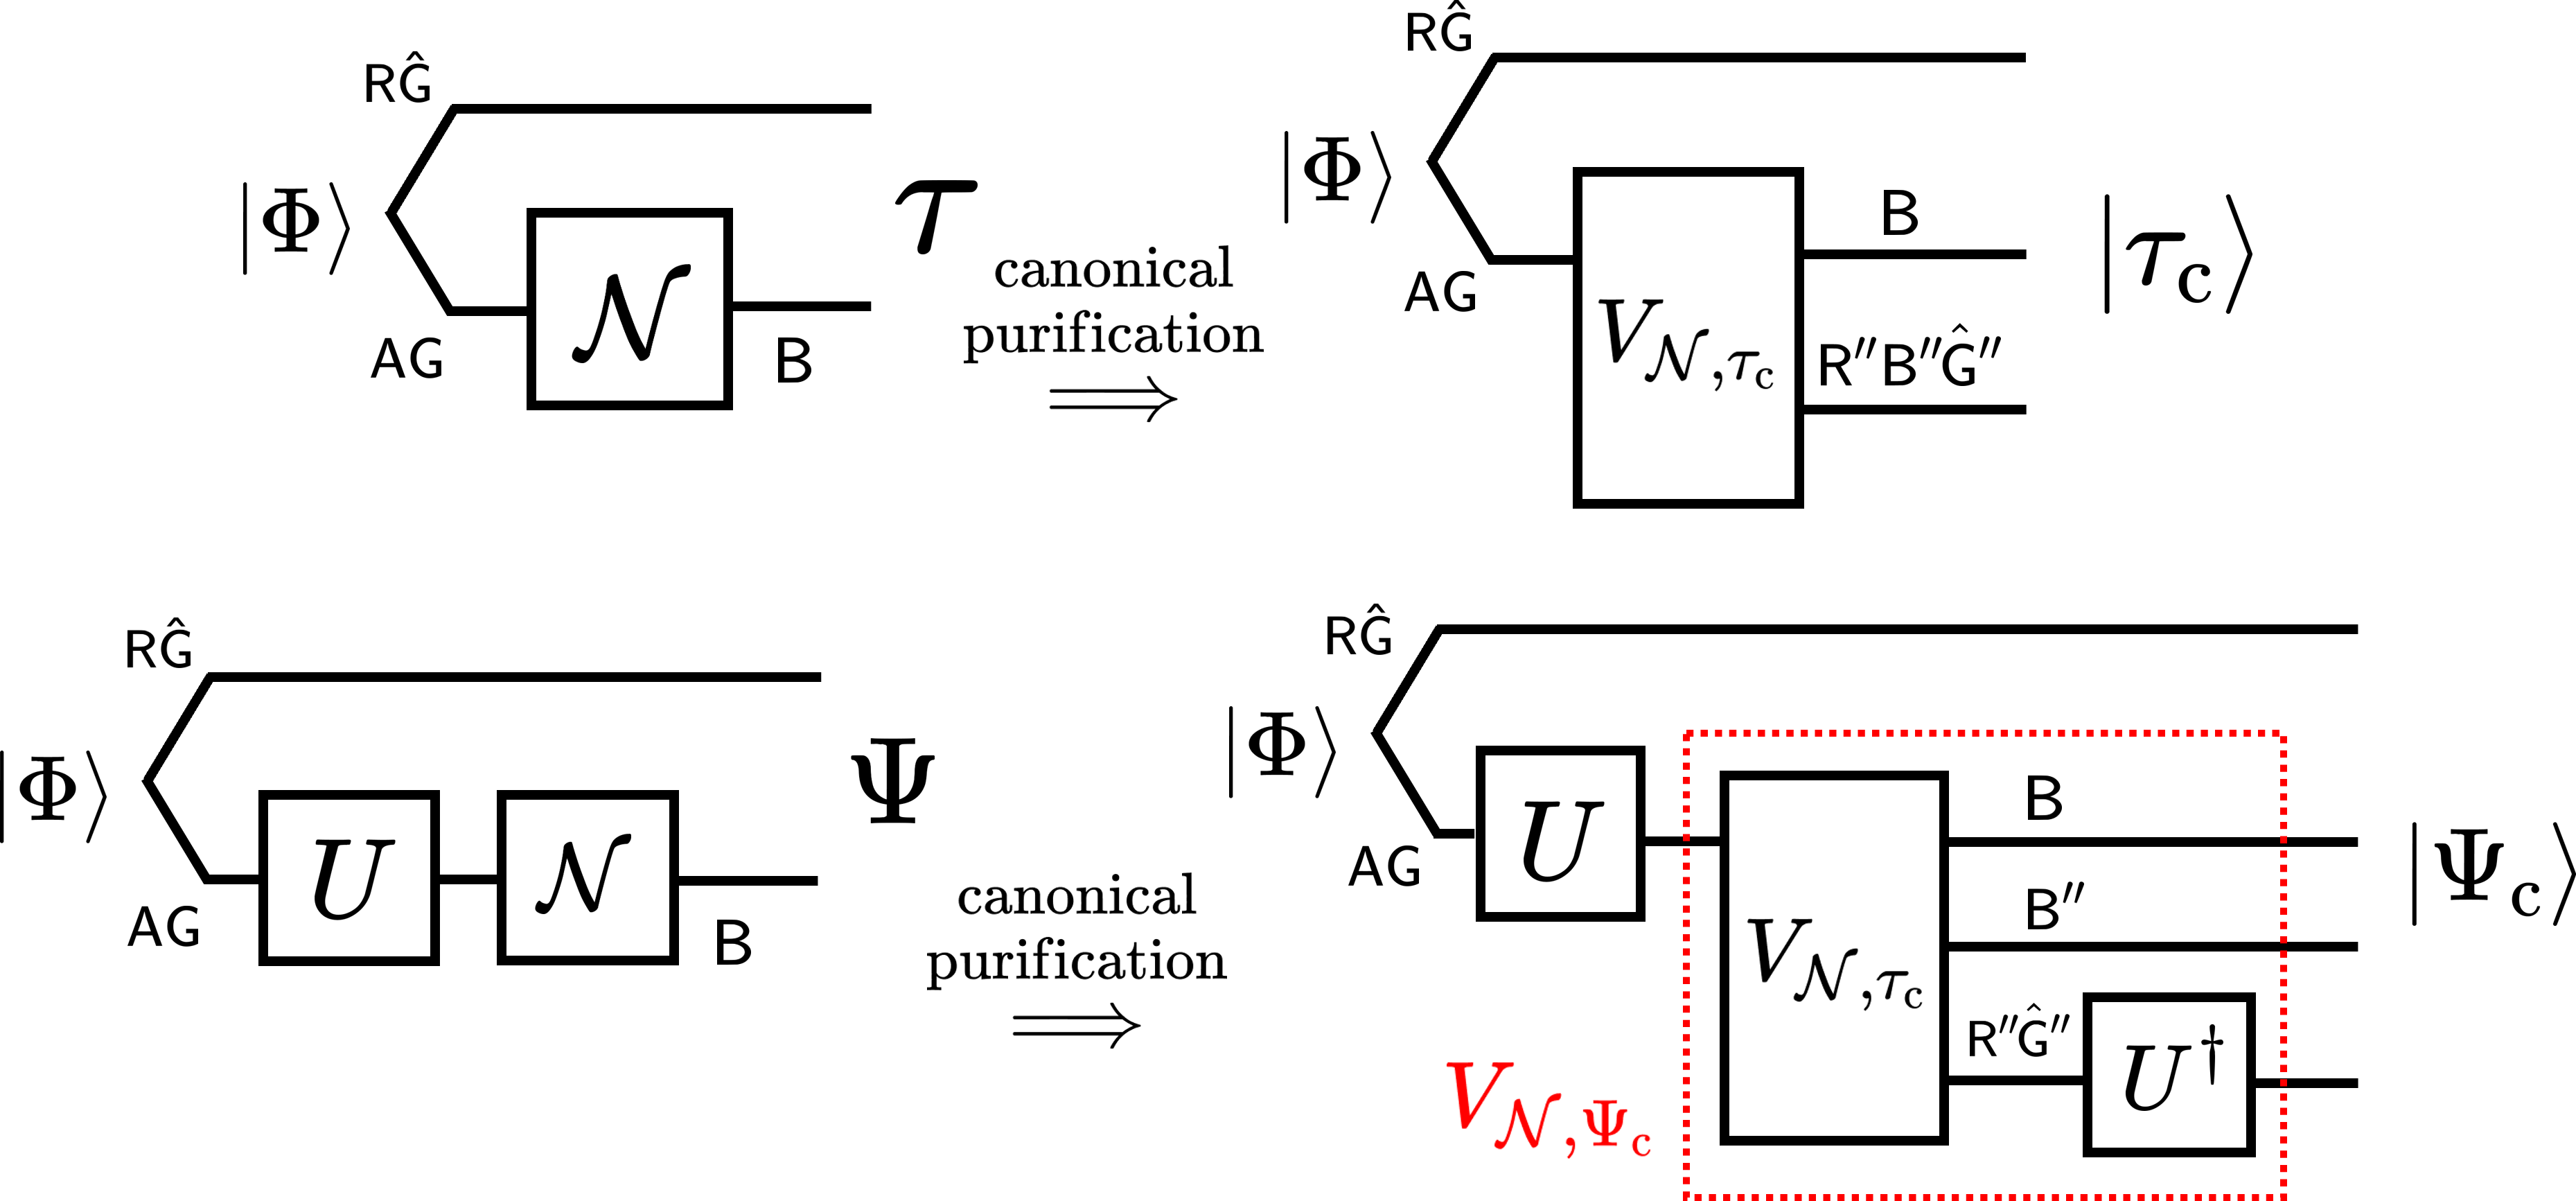
\includegraphics[width=120mm]{fig6.png}
    \caption{A diagram of the Stinespring dilation of $\cN^{\sA\sG\rarr\sB}$ induced by the canonical purification.
    We denote by $V_{\cN, \tau_{\rm c}}^{\sA\sG\rarr\sB\sR''\sB''\hat{\sG}''}$ the Stinespring isometry associated with $\ket{\tau_{\rm c}}^{\sR\sB\hat{\sG}\sR''\sB''\hat{\sG}''}$.
    Then, the Stinespring isometry corresponding to $\ket{\Psi_{\rm c}}^{\sR\sB\hat{\sG}\sR''\sB''\hat{\sG}''}$ is given by $(U^{\sR''\hat{\sG}''})^\dag V_{\cN, \tau_{\rm c}}^{\sA\sG\rarr\sB\sR''\sB''\hat{\sG}''}$, which is denoted as $V_{\cN, \Psi_{\rm c}}^{\sA\sG\rarr\sB\sR''\sB''\hat{\sG}''}$ and shown in a red dotted box.
    The complementary channels determined from these isometries are generally not identical, so Eq.~\eqref{inteq:136} cannot be applied directly.
    To resolve this issue, it suffices for Bob to apply $U^{\sR''\hat{\sG}''}$ to copies of $\ket{\Psi_{\rm c}}^{\sR\sB\hat{\sG}\sR''\sB''\hat{\sG}''}$ at hand in the algorithm, thereby canceling the extra $(U^{\sR''\hat{\sG}''})^\dag$.}
    \label{fig:dilation states}
\end{figure}



Let $\ket{\til{\Psi}_{\rm c}}^{\sR\sB\hat{\sG}\sR''\sB''\hat{\sG}''}$ be a state given by $\ket{\til{\Psi}_{\rm c}}^{\sR\sB\hat{\sG}\sR''\sB''\hat{\sG}''} = U^{\sR''\hat{\sG}''}\ket{\Psi_{\rm c}}^{\sR\sB\hat{\sG}\sR''\sB''\hat{\sG}''}$. One can check that the complementary channels associated with $\ket{\til{\Psi}_{\rm c}}^{\sR\sB\hat{\sG}\sR''\sB''\hat{\sG}''}$ and $\ket{\tau_{\rm c}}^{\sR\sB\hat{\sG}\sR''\sB''\hat{\sG}''}$ are identical: $\bar{\cN}_{\tau_{\rm c}}^{\sA\sG\rarr\sR''\sB''\hat{\sG}''} = \bar{\cN}_{\til{\Psi}_{\rm c}}^{\sA\sG\rarr\sR''\sB''\hat{\sG}''}$. We denote these channel by $\bar{\cN}_{\rm c}^{\sA\sG\rarr\sR''\sB''\hat{\sG}''}$ for simplicity.
When we construct the Uhlmann transformation $\til{V}^\sM$ from $\ket{\til{\Psi}_{\rm c}}^{\sR\sB\hat{\sG}\sR''\sB''\hat{\sG}''}$ and $\ket{\tau_{\rm c}}^{\sR\sB\hat{\sG}\sR''\sB''\hat{\sG}''}$, it holds that
\begin{align}
\label{inteq:68}
    \rF\big(\til{V}^\sM\ket{\til{\Psi}_{\rm c}}^{\sR\sB\hat{\sG}\sR''\sB''\hat{\sG}''}\ket{0}^{\hat{\sR}\hat{\sA}}, \ket{\Phi}^{\sR\hat{\sA}}\ket{\tau_{\rm c}}^{\hat{\sR}\sB\hat{\sG}\sR''\sB''\hat{\sG}''}\big)
    &= \rF\big(\bar{\cN}_{\rm c}^{\sA\sG\rarr\sR''\sB''\hat{\sG}''}\circ\cU^{\sA\sG}(\Phi^{\sR\sA} \otimes \pi^\sG), \pi^\sR\otimes \tau_{\rm c}^{\sR''\sB''\hat{\sG}''}\big) \\
    &\geq 1 -\epsilon,
\end{align}
where $\tau_{\rm c}^{\sR''\sB''\hat{\sG}''} = \bar{\cN}_{\rm c}^{\sA\sG\rarr\sR''\sB''\hat{\sG}''}(\pi^{\sA\sG})$.
The inequality is due to the decoupling condition Eq.~\eqref{inteq:136}, where $\sE = \sR''\sB''\hat{\sG}''$.
While Bob cannot act on $\sR''\hat{\sG}''$ of the \emph{actual} environment, rather than on its copies, this does not cause any issue because the environment can be arbitrarily chosen.
Note that Eq.~\eqref{inteq:136} does not depend on the particular choice of the complementary channel of $\cN^{\sA\sG\rarr\sB}$, as long as the complementary channels appearing in the first and second arguments of the fidelity on the left-hand side are identical.




Based on the above discussion, to implement the Uhlmann decoder in this model, we introduce the following two simple modifications to
Algorithm~\ref{alg:Uhl mixed sample}, $\mathtt{UhlmannMixedSample}(\Psi^{\sR'\sB'\hat{\sG}'}, \tau^{\sR'\sB'\hat{\sG}'}; \delta, \tF)$.
The first modification is to apply an additional unitary $U^{\sR''\hat{\sG}''}$ after $\mathtt{CanonicalPurification}$ of $\Psi^{\sR'\sB'\hat{\sG}'}$.
The second modification is to perform the Uhlmann transformation on $\sM = \sB\hat{\sG}\hat{\sR}\hat{\sA}$ in the step of $\mathtt{UhlmannPurifiedSample}$, which approximately maps $\ket{\til{\Psi}_{\rm c}}^{\sR\sB\hat{\sG}\sR''\sB''\hat{\sG}''}\ket{0}^{\hat{\sR}\hat{\sA}}$ to $\ket{\Phi}^{\sR\hat{\sA}}\ket{\tau_{\rm c}}^{\hat{\sR}\sB\hat{\sG}\sR''\sB''\hat{\sG}''}$.
From Theorem~\ref{thm:Uhlmann mixed state sample}, we can implement a transformation $\cT^\sM$ that satisfies 
\begin{align}
    &\rF\big(\cT^\sM(\ketbra{\til{\Psi}_{\rm c}}{\til{\Psi}_{\rm c}}^{\sR\sB\hat{\sG}\sR''\sB''\hat{\sG}''}\otimes\ketbra{0}{0}^{\hat{\sR}\hat{\sA}}), \ket{\Phi}^{\sR\hat{\sA}}\ket{\tau_{\rm c}}^{\hat{\sR}\sB\hat{\sG}\sR''\sB''\hat{\sG}''}\big) \notag\\
    &\geq \rF\big(\bar{\cN}_{\rm c}^{\sA\sG\rarr\sR''\sB''\hat{\sG}''}\circ\cU^{\sA\sG}(\Phi^{\sR\sA} \otimes \pi^\sG), \pi^\sR\otimes \tau_{\rm c}^{\sR''\sB''\hat{\sG}''}\big) - \delta\\
    \label{inteq:161}
    &\geq 1 -\epsilon -\delta,
\end{align}
using multiple copies of $\Psi^{\sR'\sB'\hat{\sG}'}$ and $\tau^{\sR'\sB'\hat{\sG}'}$, where $\tau_{\rm c}^{\sR''\sB''\hat{\sG}''} = \bar{\cN}_{\rm c}^{\sA\sG\rarr\sR''\sB''\hat{\sG}''}(\pi^{\sA\sG})$ and we used the decoupling condition Eq.~\eqref{inteq:136}.
Hence, from Eq.~\eqref{inteq:161} and the monotonicity of the fidelity under the partial trace, we obtain that a quantum channel $\til{\cD}^{\sB\hat{\sG}\rarr\hat{\sA}}$ defined by $\til{\cD}^{\sB\hat{\sG} \rarr \hat{\sA}} = \tr_{\sB\hat{\sG}\hat{\sR}} \circ \cT^\sM \circ \cP_{\ket{0}}^{\bC\rarr\hat{\sR}\hat{\sA}}$ satisfies Eq.~\eqref{inteq:157}.



The number of uses of $\cN^{\sA'\sG'\rarr\sB'}$ for implementing $\til{\cD}^{\sB\hat{\sG}\rarr\hat{\sA}}$ is evaluated as
\begin{align}
\label{inteq:140}
    &\til{\cO}\Big(\f{d_\sA d_\sB d_\sG}{\delta^2 s_{\rm min}^3} \min\Big\{\f{1}{\lambda_{\rm min}^2(\Psi^{\sR\sB\hat{\sG}})} + \f{1}{\lambda_{\rm min}^2(\tau^{\sR\sB\hat{\sG}})}, \f{d_\sA^2 d_\sB^2 d_\sG^2}{\delta^4 s_{\rm min}^4}\Big\}\Big),
\end{align}
where $s_{\rm min}$ is the minimum non-zero singular value of $\sqrt{\til{\Psi}_{\rm c}^{\sR\sR''\sB''\hat{\sG}''}}\Big(\sqrt{\pi^\sR}\otimes\sqrt{\tau_{\rm c}^{\sR''\sB''\hat{\sG}''}}\Big)$.
Finally, applying Eq.~\eqref{inteq:138} to Eq.~\eqref{inteq:140}, we obtain the result of Eq.~\eqref{inteq:137}.
Since this algorithm runs sequentially in both Model~1 and Model~2, $\cO\big(\log(d_\sA d_\sB d_\sG)\big)$ qubits suffice at any one time.




\end{proof}







%==============================================================================================================================================





\subsection{One-shot quantum state merging}
\label{sec:entdis and uhl}

As another application of the decoupling and the Uhlmann transformation, we consider quantum state merging, which is often regarded as a generalization of entanglement distillation.
In \Cref{sec:setting of state merging}, we introduce the setting, and in \Cref{sec:implement uhl in state merging}, we discuss the implementation of the Uhlmann transformation for quantum state merging using our algorithm.


\subsubsection{Setting}
\label{sec:setting of state merging}


Suppose that a state $\ket{\omega}^{\sR\sA\sB}$ is shared between Alice, Bob, and the reference $\sR$, where $\sA$ and $\sB$ are held by Alice and Bob, respectively.
Their goal is to transfer Alice's system $\sA$ of $\ket{\omega}^{\sR\sA\sB}$ to Bob using only local operations and noiseless classical communication, while simultaneously distilling as much entanglement as possible between Alice and Bob.
That is, the task is to implement the following transformation, with the size of systems $\sS$ and $\hat{\sS}$ taken as large as possible:
\begin{align}
    \cB^{\sB\sX\rarr\hat{\sA}\sB\hat{\sS}}\circ\cA^{\sA\rarr\sS\sX}(\omega^{\sR\sA\sB}) \approx \omega^{\sR\hat{\sA}\sB} \otimes \Phi^{\sS\hat{\sS}},    
\end{align}
where $\cA^{\sA\rarr\sS\sX}$ and $\cB^{\sB\sX\rarr\hat{\sA}\sB\hat{\sS}}$ are performed by Alice and Bob, respectively, and $X$ is a classical register transmitted from Alice to Bob.
In the final state, $\sS$ and $\hat{\sA}\sB\hat{\sS}$ are held by Alice and Bob, respectively.



We here follow the protocol in Refs.~\cite{horodecki2007quantum, berta2008singleshot, dupuis2014one, khatri2024principlemodern}, which we describe below.
See also \Cref{fig:diagram of ent distill}.
Alice applies $\cA^{\sA\rarr\sS\sX} = \cE^{\sA \rarr \sS\sX} \circ \cU^\sA$, where $U^\sA$ is a Haar random unitary, and 
\begin{align}
\label{eq:distill E channel}
    \cE^{\sA\rarr\sS\sX}(\cdot) = \sum_x U_x^{\sA\rarr\sS}\Pi_x^\sA(\cdot)\Pi_x^\sA(U_x^{\sA\rarr\sS})^\dag \otimes \ketbra{x}{x}^\sX.
\end{align}
The projection $\Pi_x^\sA$ is onto a $d_\sS$-dimensional subspace $\cH_x^\sA$ of $\cH^\sA$ and $U_x^{\sA\rarr \sS}$ is a partial isometry which maps the subspace $\cH_x^\sA$ to $\cH^\sS$ spanned by a fixed orthonormal basis. For simplicity, we assume $d_\sX = d_\sA/d_\sS$.





\begin{figure}
    \centering
    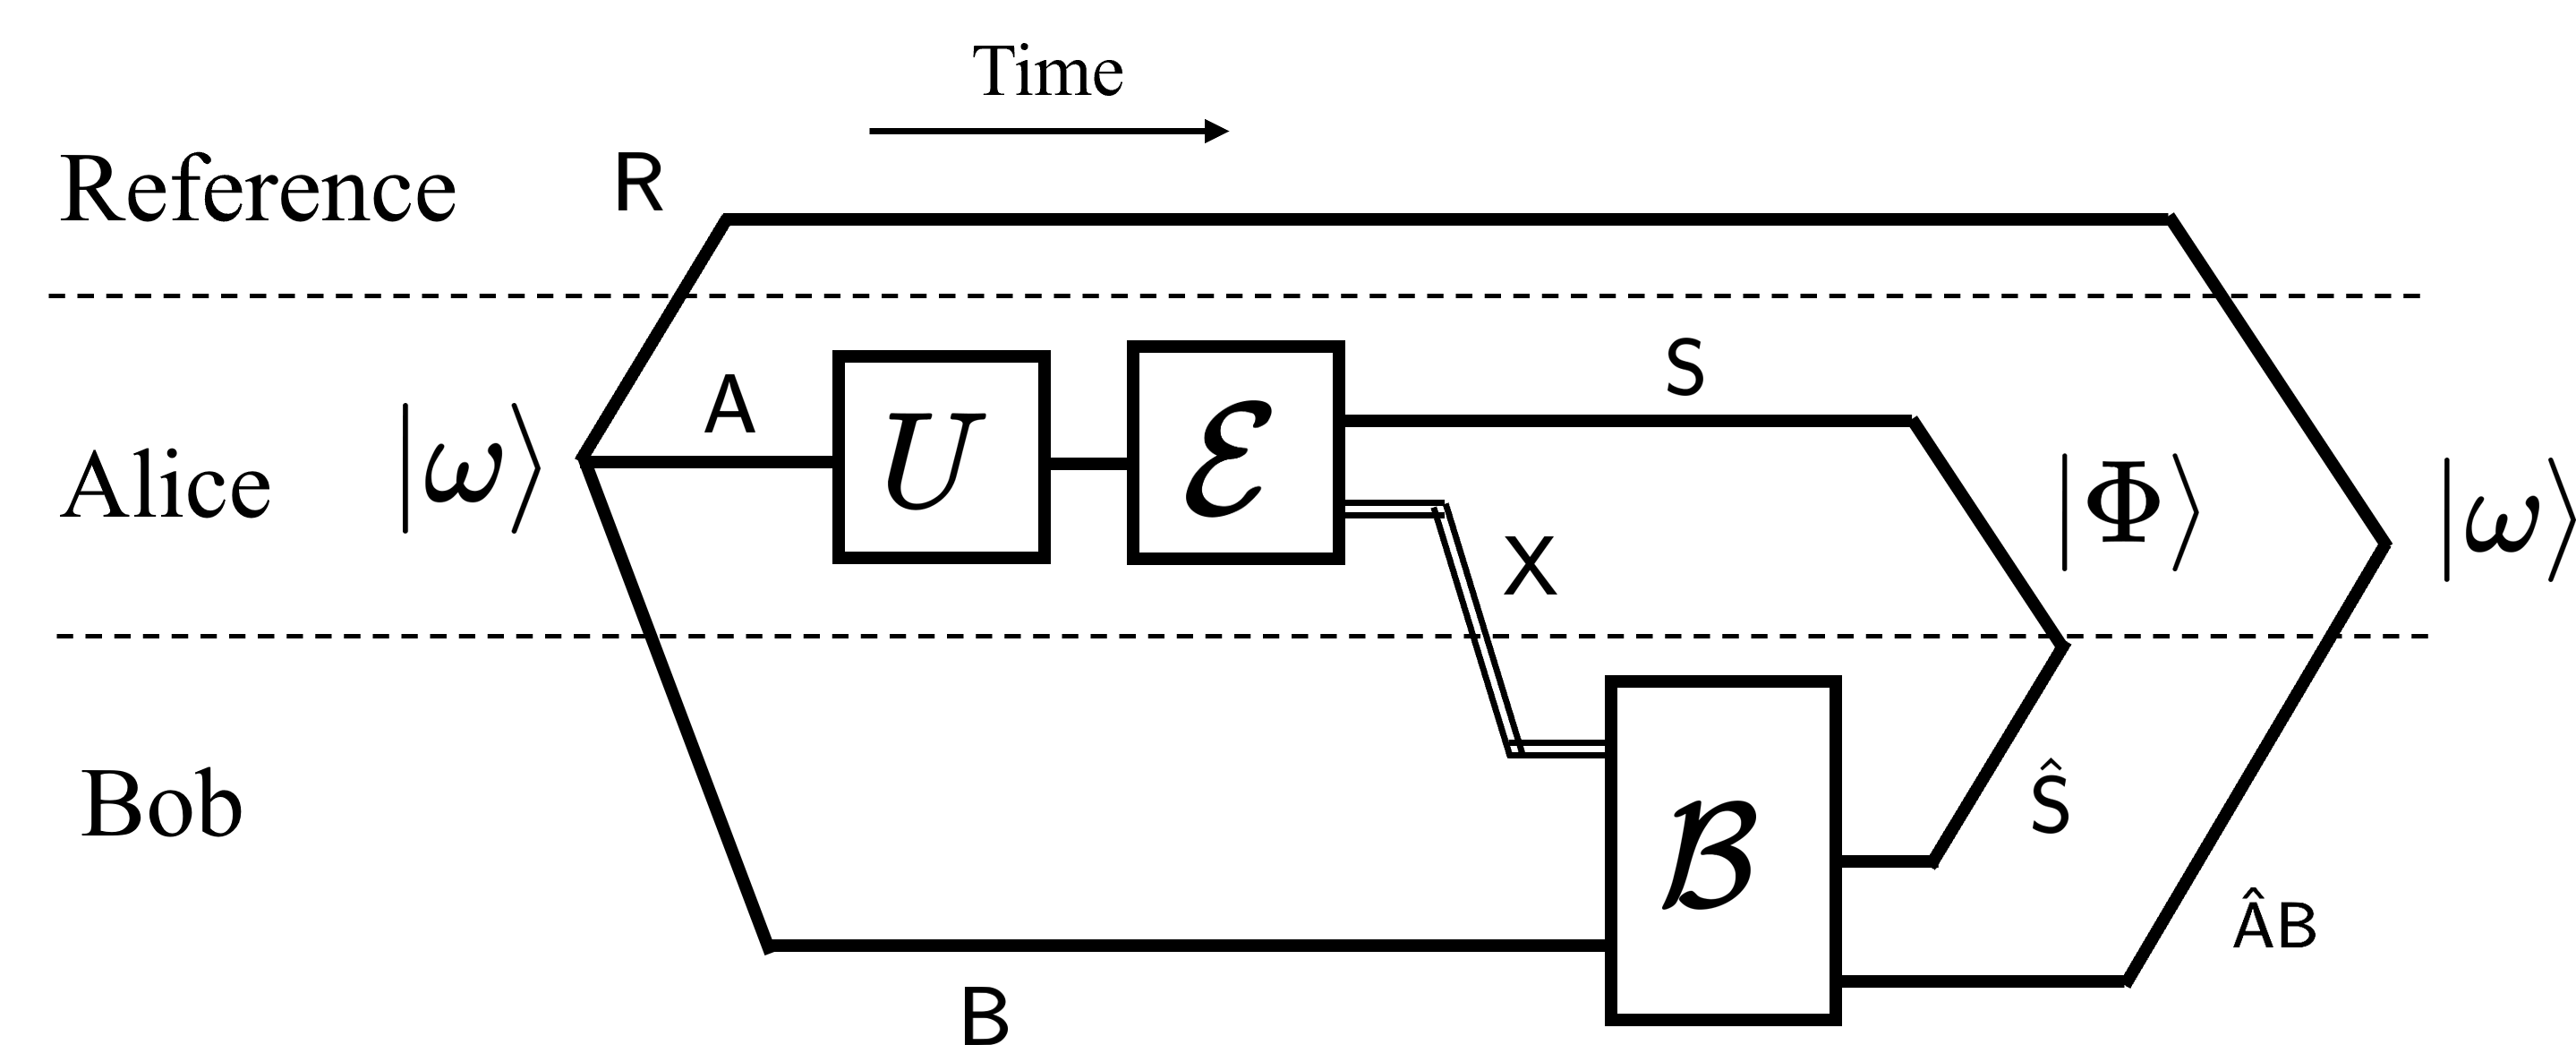
\includegraphics[width=100mm]{fig7.png}
    \caption{A diagram of quantum state merging.
    The goal is to transfer Alice's subsystem, which is part of a joint quantum state $\ket{\omega}^{\sR\sA\sB}$, to Bob, while simultaneously distilling as much entanglement as possible between $\sS$ and $\hat{\sS}$, using only local operations and classical communication.
    The double line connecting Alice and Bob represents a noiseless classical communication channel.
    }
    \label{fig:diagram of ent distill}
\end{figure}






After receiving the register $\sX$ by classical communication, which stores the measurement outcome $x$, Bob performs the operation $\cB^{\sB\sX \to \hat{\sA}\sB\hat{\sS}}$ specified as follows.
Let $\sqrt{p_x}\ket{\psi_x}^{\sR\sS\sB} = U_x^{\sA \to \sS} \Pi_x^\sA U^\sA\ket{\omega}^{\sR\sA\sB}$, where $p_x$ is the probability that the outcome $x$ occurs, and $\ket{\psi_x}^{\sR\sS\sB}$ is the resulting state.
Then, the operation $\cB^{\sB\sX \to \hat{\sA}\sB\hat{\sS}}$ is constructed as $\cB^{\sB\sX\rarr\hat{\sA}\sB\hat{\sS}} = \tr_\sX \circ \cW^{\hat{\sA}\sB\hat{\sS}\sX} \circ \cP_{\ket{0}}^{\bC\rarr\hat{\sA}\hat{\sS}}$, where $W^{\hat{\sA}\sB\hat{\sS}\sX}$ is a unitary such that $W^{\hat{\sA}\sB\hat{\sS}\sX} = \sum_x V_x^{\hat{\sA}\sB\hat{\sS}} \otimes \ketbra{x}{x}^\sX$, and $ V_x^{\hat{\sA}\sB\hat{\sS}}$ is the Uhlmann unitary satisfying 
\begin{align}
\label{inteq:111}
    \rF\big(V_x^{\hat{\sA}\sB\hat{\sS}}\ket{\psi_x}^{\sR\sS\sB}\ket{0}^{\hat{\sA}\hat{\sS}}, \ket{\omega}^{\sR\hat{\sA}\sB}\ket{\Phi}^{\sS\hat{\sS}}\big) = \rF(\psi_x^{\sR\sS}, \omega^\sR\otimes\pi^\sS).
\end{align}


We remark on the performance of the above protocol.
Let $\bar{\cE}^{\sA\rarr\sS\sE}$ be a complementary channel of $\cE^{\sA\rarr\sX} = \tr_\sS\circ\cE^{\sA\rarr\sS\sX}$, where $\sE$ is an environment of the classical channel from Alice to Bob.
We assume $d_\sE = d_\sX$ without loss of generality.
The decoupling theorem~\cite{dupuis2014one} ensures that the Haar random unitary $U^\sA$ satisfies
\begin{align}
\label{eq:OneShotDecouplingExpectDistill}
    \rF\big(\bar{\cE}^{\sA\rarr\sS\sE}\circ\cU^\sA(\omega^{\sR\sA}), \omega^\sR \otimes \pi^\sS \otimes \pi^\sE \big) \geq 1 - \epsilon,
\end{align}
with high probability.
Here, $\epsilon$ can be taken sufficiently small, depending on the properties of the initial state $\ket{\omega}^{\sR\sA\sB}$ and the channel $\cE^{\sA\rarr\sS\sX}$, such as the dimension of the system $\sS$ and the amount of initial entanglement between the systems $\sA$ and $\sB$~\cite{dupuis2014one}.
In Eq.~\eqref{eq:OneShotDecouplingExpectDistill}, the reduced Choi--Jamio\l kowski state on $\sS\sE$ is given by $\bar{\cE}^{\sA\rarr\sS\sE}(\pi^\sA) = \pi^\sS \otimes \pi^\sE$.
This is because, according to the outcome $x$, each $U_x^{\sA\rarr\sS}$ maps from $\cH_x^\sA$ to $\cH^\sS$, which is spanned by a fixed basis, and thus, $U_x^{\sA\rarr \sS}\Pi_x^\sA(U_x^{\sA\rarr\sS})^\dag$ is independent of $x$ and equals $\bI^\sS$.
Then, under the decoupling condition Eq.~\eqref{eq:OneShotDecouplingExpectDistill}, it is known that the operation $\cB^{\sB\sX\rarr\hat{\sA}\sB\hat{\sS}}$ achieves the task of quantum state merging with fidelity at least $1-\epsilon$. For details, see, e.g., Ref.~\cite{khatri2024principlemodern}.



%========================================================================================================================================================================================================================================





\subsubsection{Algorithmic implementation of Bob's operation based on the Uhlmann transformation}
\label{sec:implement uhl in state merging}


We consider explicitly implementing the unitary $W^{\hat{\sA}\sB\hat{\sS}\sX} = \sum_x V_x^{\hat{\sA}\sB\hat{\sS}} \otimes \ketbra{x}{x}^\sX$, using our Uhlmann transformation algorithm.
In this case, the Uhlmann unitary $V_x^{\hat{\sA}\sB\hat{\sS}}$ is conditioned by $x$ and should be realized for all $x$.
For algorithmic construction, we assume that Bob has full knowledge of Alice's operation $\cA^{\sA\rarr\sS\sX} = \cE^{\sA\rarr\sS\sX}\circ\cU^\sA$ and is capable of implementing it. 
While $U^\sA$ is chosen uniformly at random by Alice, Bob can identify the unitary Alice chose, for instance, using shared randomness.

We address the following model: 
\begin{itemize}
    \item A model in which multiple independent and identical copies of the initial state, $\ket{\omega}^{\sR'\sA'\sB'}$, are available.
\end{itemize}
We then evaluate the number of samples of $\ket{\omega}^{\sR'\sA'\sB'}$ required for Bob's operation.
We should distinguish the systems used by Bob, e.g., $\sR'$ and $\sA'$, from those that already exist as the reference $\sR$ and Alice's systems $\sA$.
The state $\ket{\omega}^{\sR'\sA'\sB'}$ is sampled and used \emph{locally} by Bob.
It is noteworthy that, in this model, Bob does not need to know a complete description of the initial state $\ket{\omega}^{\sR\sA\sB}$; rather, Bob is provided with copies of the state, whose description remains unknown to Bob.




We define a state $\ket{\Psi}^{\sR\sS\sB\sX\sE} = V_\cA^{\sA\rarr\sS\sX\sE}\ket{\omega}^{\sR\sA\sB}$, where $V_\cA^{\sA\rarr\sS\sX\sE}$ is a Stinespring isometry of $\cA^{\sA\rarr\sS\sX} = \cE^{\sA\rarr\sS\sX}\circ \cU^\sA$. 
We introduce $m_{\rm min}$ and $r_{\rm max}$ as  
\begin{align}
    \label{inteq:142}
    m_{\rm min} = \min_x\Big[\f{p_x}{d_\sX}s_{\rm min}\Big(\sqrt{\psi_x^{\sR\sS}}\big(\sqrt{\omega^\sR}\otimes\sqrt{\pi^\sS}\big)\Big)\Big], \ \ \ \text{and} \ \ \ r_{\rm max} = \max_x\Big[r\Big(\sqrt{\psi_x^{\sR\sS}}\big(\sqrt{\omega^\sR}\otimes\sqrt{\pi^\sS}\big)\Big)\Big],
\end{align}
where $s_{\rm min}(\cdot)$ and $r(\cdot)$ are the minimum non-zero singular value and the rank of an input matrix, respectively.
The maximization and minimization are taken over all outcomes $x$.


Our statement is as follows. 

\begin{theorem}[Uhlmann transformation algorithm in quantum state merging]
\label{thm:Uhlmann state merging}
    In the setting of quantum state merging, suppose that for some $\epsilon \in [0, 1]$,  
    \begin{align}
    \label{inteq:141}
            \rF\big(\Psi^{\sR\sS\sE}, \omega^\sR \otimes \pi^\sS \otimes \pi^\sE \big) \geq 1 - \epsilon.
    \end{align}
    Then, for $\delta \in (0, 1)$, there exists a quantum algorithm that implements a quantum channel $\til{\cB}^{\sB\sX\rarr\hat{\sA}\sB\hat{\sS}}$, which satisfies
    \begin{align}
        \rF\big(\til{\cB}^{\sB\sX\rarr\hat{\sA}\sB\hat{\sS}}(\Psi^{\sR\sS\sB\sX}), \ket{\omega}^{\sR\hat{\sA}\sB}\ket{\Phi}^{\sS\hat{\sS}}\big) \geq 1 - \epsilon - \delta,
    \end{align}
    using $\zeta$ samples of $\ket{\omega}^{\sR'\sA'\sB'}$, where $\zeta = \cO\Big(\f{1}{\delta^2}\min\Big\{\f{1}{m_{\rm min}^2}, \f{r_{\rm max}^2}{\delta^4}\Big\}\Big(\log{\Big(\f{1}{\delta}\Big)}\Big)^2\Big)$, and $m_{\rm min}$ and $r_{\rm max}$ are given by Eqs.~\eqref{inteq:142}. The quantum circuit for the algorithm consists of $\cO\big(\zeta\log{(d_\sR d_\sA d_\sB)}\big)$ one- and two-qubit gates, and $\cO\big(\log{(d_\sR d_\sA d_\sB)}\big)$ qubits suffice at any one time.
\end{theorem}



This theorem states that when $\Psi^{\sR\sS\sX}$ is sufficiently decoupled as $\Psi^{\sR\sS\sX} \approx \omega^\sR \otimes \pi^\sS \otimes \pi^\sX$ by Alice's operation, then by taking small $\delta$ and applying $\til{\cB}^{\sB\sX\rarr\hat{\sA}\sB\hat{\sS}}$---which is explicitly constructed using our algorithm---Bob can accomplish the task of quantum state merging.




\begin{proof}[Proof of Theorem~\ref{thm:Uhlmann state merging}]
    


Let $\sL = \sR\sS$ and $\sM = \hat{\sA}\sB\hat{\sS}$. 
We define $\ket{\sigma}^{\sL\sM}$ and $\Psi^{\sL\sM\sX}$ by $\ket{\sigma}^{\sL\sM} = \ket{\omega}^{\sR\hat{\sA}\sB}\ket{\Phi}^{\sS\hat{\sS}}$ and 
\begin{align}
    \Psi^{\sL\sM\sX} 
    &= \cP_{\ket{0}}^{\bC\rarr\hat{\sA}\hat{\sS}} \circ \cE^{\sA\rarr\sS\sX}\circ\cU^\sA(\ketbra{\omega}{\omega}^{\sR\sA\sB}) \\
    &= \sum_x  p_x\ketbra{\psi_x}{\psi_x}^{\sR\sS\sB} \otimes \ketbra{x}{x}^{\sX} \otimes \ketbra{0}{0}^{\hat{\sA}\hat{\sS}} \\
    &= \sum_x  p_x\ketbra{\rho_x}{\rho_x}^{\sL\sM} \otimes \ketbra{x}{x}^{\sX},
\end{align}
where $\ket{\rho_x}^{\sL\sM} = \ket{\psi_x}^{\sR\sS\sB}\ket{0}^{\hat{\sA}\hat{\sS}}$.
We then consider 
\begin{align}
    \cJ^{\sM\sH\hat{\sL}\hat{\sM}\sX} 
    = \mathtt{UhlmannPurifiedSample}(\Psi^{\sL'\sM'\sX'}, \sigma^{\sL'\sM'}\otimes\pi^{\sX'}; \delta_1, \tF),
\end{align}
where $\hat{\sL}$ and $\hat{\sM}$ are auxiliary systems of the same number of qubits as $\sL$ and $\sM$, respectively. 
Here, the inputs to $\mathtt{UhlmannPurifiedSample}$ are mixed states. This aims to transform $\ket{\rho_x}^{\sL\sM}$ to $\ket{\sigma}^{\sL\sM}$ for all $x$ by acting on $\sM\sX$.
The procedure and performance analysis of this channel is a direct extension of the one in \Cref{alg:Uhl purif sample} and Theorem~\ref{thm:algorithm Uhlmann}.


The quantum channel $\cJ^{\sM\sH\hat{\sL}\hat{\sM}\sX}$ satisfies 
\begin{align}
\label{inteq:133}
    \f{1}{2}\big\|\cJ^{\sM\sH\hat{\sL}\hat{\sM}\sX} - \cU_1^{\sM\sH\hat{\sL}\hat{\sM}\sX}\big\|_\diamond \leq \delta_1/2,
\end{align}
where $U_1^{\sM\sH\hat{\sL}\hat{\sM}\sX}$ is a block-encoding unitary of $\sum_x \ketbra{\rho_x}{\sigma}^{\hat{\sL}\hat{\sM}} \otimes \til{V}_x^\sM \otimes \ketbra{x}{x}^\sX$, $\til{V}_x^\sM = P_\sgn^{(\rm SV)}\big(\sin^{(\rm SV)}(M_x^\sM)\big)$, and $M_x^\sM = \f{p_x}{d_\sX} \tr_\sL[\ket{\sigma}\bra{\rho_x}^{\sL\sM}]$. (See also Eq.~\eqref{inteq:16} with rescaling by $\delta_2 \gets \delta_1/(2u)$).


Let $m_{\rm min}$ and $r_{\rm max}$ be defined by 
\begin{align}
\label{inteq:118}
    m_{\rm min}
    &= \min_x \big[s_{\rm min}(M_x^\sM)\big] \\
    &= \min_x \Big[\sqrt{\f{p_x}{d_\sX}}s_{\rm min}\Big(\sqrt{\Psi^{\sR\sS\sX}}\big(\sqrt{\omega^\sR}\otimes\sqrt{\pi^\sS}\otimes\pi^\sX\big)\Big)\Big] \\
    &= \min_x\Big[\f{p_x}{d_\sX}s_{\rm min}\Big(\sqrt{\psi_x^{\sR\sS}}\big(\sqrt{\omega^\sR}\otimes\sqrt{\pi^\sS}\big)\Big)\Big],
\end{align}
where $\Psi^{\sR\sS\sX} = \cE^{\sA\rarr\sS\sX}\circ\cU^\sA(\omega^{\sR\sA})$, and
\begin{align}
\label{inteq:119}
    r_{\rm max} 
    &= \max_x\big[r(M_x^\sM)\big] \\
    &= \max_x\Big[r\Big(\sqrt{\psi_x^{\sR\sS}}\big(\sqrt{\omega^\sR}\otimes\sqrt{\pi^\sS}\big)\Big)\Big],
\end{align}
where $s_{\rm min}(\cdot)$ and $r(\cdot)$ denote the minimum non-zero singular value and the rank of an input matrix, respectively.
The maximization and minimization over $x$ are crucial to ensure that the algorithm covers all $x$.


From the discussion in \Cref{sec:uhlfidpurifsamp} (especially, from Eq.~\eqref{inteq:120} to Eq.~\eqref{inteq:51} with rescaling by $\delta_1 \gets \delta_1/8$), when we set $\beta = \cO(\max\{m_{\rm min}, \delta_1/r_{\rm max}\})$, it holds that, for all $x$, 
\begin{align}
\label{inteq:113}
    \big|\sqrt{\rF}(\til{V}_x^\sM\ket{\rho_x}^{\sL\sM}, \ket{\sigma}^{\sL\sM}) - \sqrt{\rF}(V_x^\sM\ket{\rho_x}^{\sL\sM}, \ket{\sigma}^{\sL\sM})\big| \leq \delta_1/4.
\end{align}
Note that the Uhlmann partial isometry $V_x^\sM$ that satisfies Eq.~\eqref{inteq:111} is given by $V_x^\sM = \sgn^{(\rm SV)}\big(\sin^{(\rm SV)}(M_x^\sM)\big)$.



Let Bob's operation $\til{\cB}^{\sB\sX\rarr\hat{\sA}\sB\hat{\sS}}$ be given by  
\begin{align}
    \til{\cB}^{\sB\sX\rarr\hat{\sA}\sB\hat{\sS}} = \tr_{\sH\hat{\sL}\hat{\sM}\sX}\circ\cJ^{\sM\sH\hat{\sL}\hat{\sM}\sX}\circ\cP_{\ket{\sigma}}^{\bC\rarr\hat{\sL}\hat{\sM}}\circ\cP_{\ket{0}}^{\bC\rarr\sH\hat{\sA}\hat{\sS}}.
\end{align}
We then evaluate the fidelity between the state obtained by applying Alice's and Bob's operations to the initial state $\ket{\omega}^{\sR\sA\sB}$ and the target state $\ket{\sigma}^{\sL\sM} = \ket{\omega}^{\sR\hat{\sA}\sB}\ket{\Phi}^{\sS\hat{\sS}}$.
To this end, we define the following states:
\begin{align}
    &\xi^{\sL\sM\sH\hat{\sL}\hat{\sM}\sX} = \cJ^{\sM\sH\hat{\sL}\hat{\sM}\sX}\circ\cP_{\ket{\sigma}}^{\bC\rarr\hat{\sL}\hat{\sM}}\circ\cP_{\ket{0}}^{\bC\rarr\sH} (\Psi^{\sL\sM\sX}), \\
    &\xi_1^{\sL\sM\sH\hat{\sL}\hat{\sM}\sX} = \cU_1^{\sM\sH\hat{\sL}\hat{\sM}\sX}\circ\cP_{\ket{\sigma}}^{\bC\rarr\hat{\sL}\hat{\sM}}\circ\cP_{\ket{0}}^{\bC\rarr\sH} (\Psi^{\sL\sM\sX}), \\
    &\xi_{\rm ideal}^{\sL\sM\sH\hat{\sL}\hat{\sM}\sX} = \cU_{\rm ideal}^{\sM\sH\hat{\sL}\hat{\sM}\sX}\circ\cP_{\ket{\sigma}}^{\bC\rarr\hat{\sL}\hat{\sM}}\circ\cP_{\ket{0}}^{\bC\rarr\sH} (\Psi^{\sL\sM\sX}),
\end{align}
where $U_{\rm ideal}^{\sM\sH\hat{\sL}\hat{\sM}\sX}$ is the exact block-encoding unitary of $\sum_x \ketbra{\rho_x}{\sigma}^{\hat{\sL}\hat{\sM}}\otimes V_x^\sM \otimes\ketbra{x}{x}^\sX$.
We further define a reference state by
\begin{align}
    \phi_{\rm ref}^{\sL\sM\sH\hat{\sL}\hat{\sM}\sX} = \sum_x \f{1}{d_\sX}\ketbra{\rho_x}{\rho_x}^{\hat{\sL}\hat{\sM}} \otimes \ketbra{\sigma}{\sigma}^{\sL\sM} \otimes \ketbra{x}{x}^\sX \otimes \ketbra{0}{0}^\sH.
\end{align}

Let $\sN = \sL\sM\sH\hat{\sL}\hat{\sM}\sX$.
We first see that
\begin{align}
    \big|\sqrt{\rF}\big(\xi_1^\sN, \phi_{\rm ref}^\sN\big) - \sqrt{\rF}\big(\xi_{\rm ideal}^\sN, \phi_{\rm ref}^\sN\big)\big| 
    &= \Big|\sum_x\sqrt{\f{p_x}{d_\sX}}\sqrt{\rF}(\til{V}_x^\sM\ket{\rho_x}^{\sL\sM}, \ket{\sigma}^{\sL\sM}) - \sum_x\sqrt{\f{p_x}{d_\sX}}\sqrt{\rF}(V_x^\sM\ket{\rho_x}^{\sL\sM}, \ket{\sigma}^{\sL\sM})\Big| \\
    &\leq \sum_x\sqrt{\f{p_x}{d_\sX}}\big|\sqrt{\rF}(\til{V}_x^\sM\ket{\rho_x}^{\sL\sM}, \ket{\sigma}^{\sL\sM}) - \sqrt{\rF}(V_x^\sM\ket{\rho_x}^{\sL\sM}, \ket{\sigma}^{\sL\sM})\big| \\
    &\leq \f{\delta_1}{4}\sum_x\sqrt{\f{p_x}{d_\sX}} \\
    \label{inteq:114}
    &\leq \f{\delta_1}{4},
\end{align}
where we used Eq.~\eqref{inteq:113} in the second inequality and $\sum_x\sqrt{\f{p_x}{d_\sX}} \leq \sqrt{\sum_x p_x} = 1$ in the lase inequality.

Next, we observe that
\begin{align}
    \big|\sqrt{\rF}\big(\xi^\sN, \phi_{\rm ref}^\sN\big) - \sqrt{\rF}\big(\xi_1^\sN, \phi_{\rm ref}^\sN\big)\big|
    &= \Big| \Big\|\sqrt{\xi^\sN}\sqrt{\phi_{\rm ref}^\sN}\Big\|_1 -  \Big\|\sqrt{\xi_1^\sN}\sqrt{\phi_{\rm ref}^\sN}\Big\|_1\Big| \\
    &\leq \Big\| \sqrt{\xi^\sN}\sqrt{\phi_{\rm ref}^\sN} - \sqrt{\xi_1^\sN}\sqrt{\phi_{\rm ref}^\sN} \Big\|_1 \\
    &\leq \Big\|\sqrt{\xi^\sN} - \sqrt{\xi_1^\sN}\Big\|_2 \Big\|\sqrt{\phi_{\rm ref}^\sN}\Big\|_2 \\
    &\leq \big\|\xi^\sN - \xi_1^\sN\big\|_1^{1/2} \\
    &\leq \big\|\cJ^\sN - \cU_1^\sN \big\|_\diamond^{1/2} \\
    \label{inteq:115}
    &\leq \sqrt{\delta_1},
\end{align}
where we used the H\"{o}lder's inequality in Eq.~~\eqref{eq:Holder ineq} in the second inequality, and Eq.~\eqref{inteq:133} in the last inequality. The third inequality follows from $\Big\|\sqrt{\phi_{\rm ref}^\sN}\Big\|_2 = 1$ and the Powers--St\o rmer inequality in Eq.~\eqref{eq:powers stormer ineq}.
From Eqs.~\eqref{inteq:114} and~\eqref{inteq:115}, we obtain that
\begin{align}
\label{inteq:116}
    \big|\sqrt{\rF}\big(\xi^\sN, \phi_{\rm ref}^\sN\big) - \sqrt{\rF}\big(\xi_{\rm ideal}^\sN, \phi_{\rm ref}^\sN\big)\big| \leq \delta_1/4 + \sqrt{\delta_1}.
\end{align}



Using the above results, we can bound the fidelity between the final state $\Psi_{\rm fin}^{\sR\hat{\sA}\sB\sS\hat{\sS}} = \til{\cB}^{\sB\sX\rarr\hat{\sA}\sB\hat{\sS}}\circ\cA^{\sA\rarr\sS\sX}(\omega^{\sR\sA\sB})$ and the target state $\ket{\omega}^{\sR\hat{\sA}\sB}\ket{\Phi}^{\sS\hat{\sS}}$ as
\begin{align}
    \sqrt{\rF}\big(\Psi_{\rm fin}^{\sR\hat{\sA}\sB\sS\hat{\sS}}, \ket{\omega}^{\sR\hat{\sA}\sB}\ket{\Phi}^{\sS\hat{\sS}}) 
    &\geq \sqrt{\rF}\big(\xi^\sN, \phi_{\rm ref}^{\sN}\big) \\
    &\geq \sqrt{\rF}\big(\xi_{\rm ideal}^\sN, \phi_{\rm ref}^\sN\big) - \delta_1/4 - \sqrt{\delta_1} \\
    &= \sum_x \sqrt{\f{p_x}{d_\sX}}\sqrt{\rF}\big(V_x^\sM\ket{\rho_x}^{\sL\sM}, \ket{\sigma}^{\sL\sM}\big) - \delta_1/4 - \sqrt{\delta_1} \\
    &= \sum_x \sqrt{\f{p_x}{d_\sX}}\sqrt{\rF}(\psi_x^{\sR\sS}, \omega^\sR \otimes \pi^\sS) - \delta_1/4 - \sqrt{\delta_1} \\
    &= \sqrt{\rF}(\Psi^{\sR\sS\sE}, \omega^\sR \otimes \pi^\sS \otimes \pi^\sE) - \delta_1/4 - \sqrt{\delta_1},
\end{align}
where we used the fact that $\tr_{\sH\hat{\sL}\hat{\sM}\sX}[\xi^\sN] = \Psi_{\rm fin}^{\sR\hat{\sA}\sB\sS\hat{\sS}}$ and $\tr_{\sH\hat{\sL}\hat{\sM}\sX}[\phi_{\rm ref}^\sN] = \sigma^{\sL\sM} = \omega^{\sR\hat{\sA}\sB}\otimes\Phi^{\sS\hat{\sS}}$ in the first inequality.
We further applied Eq.~\eqref{inteq:116} in the second inequality and Eq.~\eqref{inteq:111} in the second equation.
Thus, noting that fidelity is always less than or equal to one, we have
\begin{align}
    \rF\big(\Psi_{\rm fin}^{\sR\hat{\sA}\sB\sS\hat{\sS}}, \ket{\omega}^{\sR\hat{\sA}\sB} \ket{\Phi}^{\sS\hat{\sS}}\big)
    &\geq \rF(\Psi^{\sR\sS\sE}, \omega^\sR \otimes \pi^\sS \otimes \pi^\sE) - 2(\delta_1/4 + \sqrt{\delta_1}) \\
    \label{inteq:112}
    &\geq 1 - \epsilon - 2(\delta_1/4 + \sqrt{\delta_1}),
\end{align}
where the last inequality follows from the condition Eq.~\eqref{inteq:141}.
Rescaling $\delta_1$ as $\delta_1 = (2\delta/5)^2$, we have $2(\delta_1/4 + \sqrt{\delta_1}) \leq \delta$.
Hence, since $\Psi_{\rm fin}^{\sR\hat{\sA}\sB\sS\hat{\sS}} = \til{\cB}^{\sB\sX\rarr\hat{\sA}\sB\hat{\sS}}\circ\cA^{\sA\rarr\sS\sX}(\omega^{\sR\sA\sB})$, we finally obtain 
\begin{align}
    \rF\big(\til{\cB}^{\sB\sX\rarr\hat{\sA}\sB\hat{\sS}}\circ\cA^{\sA\rarr\sS\sX}(\omega^{\sR\sA\sB}), \ket{\omega}^{\sR\hat{\sA}\sB} \ket{\Phi}^{\sS\hat{\sS}}\big) \geq 1 - \epsilon - \delta.
\end{align}



From Theorem~\ref{thm:algorithm Uhlmann}, the number of samples of $\Psi^{\sL'\sM'\sX'}$ and $\sigma^{\sL'\sM'}\otimes\pi^{\sX'}$ for implementing 
\begin{align}
    \mathtt{UhlmannPurifSample}(\Psi^{\sL'\sM'\sX'}, \sigma^{\sL'\sM'}\otimes\pi^{\sX'}; \delta_1, \tF) 
\end{align}
is given by $\cO\Big(\big(\log{(1/\delta_1)}\big)^2/(\delta_1\beta^2)\Big)$. 
Both $\Psi^{\sL'\sM'\sX'}$ and $\sigma^{\sL'\sM'}$ are prepared from a single copy of $\ket{\omega}^{\sR'\sA'\sB'}$. 
Recalling that $\beta = \cO(\max\{m_{\rm min}, \delta_1/r_{\rm max}\})$ and $\delta_1 \leq (2\delta/5)^2$, we evaluate the number of samples of $\ket{\omega}^{\sR'\sA'\sB'}$ for Bob's operation $\til{\cB}^{\sB\sX \rarr\hat{\sA}\sB\hat{\sS}}$ as
\begin{align}
    \zeta 
    &= \cO\Big(\f{1}{\delta_1\beta^2}\Big(\log{\Big(\f{1}{\delta_1}\Big)}\Big)^2\Big) \notag\\
    &= \cO\Big(\f{1}{\delta^2}\min\Big\{\f{1}{m_{\rm min}^2}, \f{r_{\rm max}^2}{\delta^4}\Big\}\Big(\log{\Big(\f{1}{\delta}\Big)}\Big)^2\Big),
\end{align}
where $m_{\rm min}$ and $r_{\rm max}$ are given by Eqs.~\eqref{inteq:118} and~\eqref{inteq:119}, respectively.
The quantum circuit of overall this algorithm includes $\cO\big(\zeta\log{(d_\sR d_\sA d_\sB)}\big)$ one- and two-qubit gates, and $\cO\big(\log{(d_\sR d_\sA d_\sB)}\big)$ qubits at any one time.




\end{proof}















%===============================================================================================================================================










